The fitter and background subtraction procedure, introduced in \Cref{sec:fitting_setup,sec:background_subtraction},
have been thoroughly validated in \Cref{sec:MC_validation} -- in simulation.
The real challenge, as usual, is ensuring that the conclusions and results observed in simulation will generalise correctly to real Belle II data.
The key concept of a blinded analysis dictates that one must validate the analysis procedure in control samples or regions -- collections of data that are abundant, well-understood and provide insight to the behaviour of signal in the detector.
In this Section, the discussion about \FEI validation, \piz and $\eta$ veto validation, photon detection efficiency and background modelling will be presented.

\begin{table}[htbp!]
    \centering
    \caption{\label{tab:correction_table} The corrections for background (and later -- signal) efficiency in the hadronic-tagged \BtoXsgamma photon-energy spectrum measurement.
    \FEI calibration calculations are discussed in \Cref{sec:fei_calibration}.
    Derivation of correction for the \piz and \eta veto are presented in \Cref{sec:piz_eta_calibration}.
    The photon detection efficiency study is described in \Cref{sec:photon_efficiency}.
    Background modelling corrections are calculated in XXXX.
    The \FEI, \piz and \gamma corrections are averaged values corresponding to the respective \EB bin,
    as the event-level information is lost after estimating good tag-\B counts using the \Mbc fit and performing the leftover-\BB background subtraction.
    \todo[inline]{figure out where this table goes.}
    }
    \resizebox{1\textwidth}{!}{
    \begin{tabular}{cccc}
        \hline
        {} \EB, GeV  & FEI calibration & \piz veto correction & \g efficiency correction\\
        \hline
        1.4-1.6  &  \multirow{11}{*}{$0.6630 \pm 0.0229$} & $1.090 \pm 0.050$ & $0.991 \pm 0.023$ \\
        1.6-1.8  &                                        & $1.074 \pm 0.048$ & $0.995 \pm 0.022$ \\
        1.8-2.0  &                                        & $1.064 \pm 0.046$ & $0.996 \pm 0.021$ \\
        2.0-2.1  &                                        & $1.055 \pm 0.046$ & $0.996 \pm 0.021$ \\
        2.1-2.2  &                                        & $1.050 \pm 0.047$ & $0.997 \pm 0.021$ \\
        2.2-2.3  &                                        & $1.046 \pm 0.047$ & $0.997 \pm 0.021$ \\
        2.3-2.4  &                                        & $1.045 \pm 0.047$ & $1.000 \pm 0.020$ \\
        2.4-2.5  &                                        & $1.047 \pm 0.047$ & $1.001 \pm 0.019$ \\
        2.5-2.6  &                                        & $1.050 \pm 0.047$ & $1.001 \pm 0.019$ \\
        2.6-2.7  &                                        & $1.050 \pm 0.046$ & $0.998 \pm 0.019$ \\
        2.7-     &                                        & $1.053 \pm 0.046$ & $0.998 \pm 0.018$ \\
        \hline
        \end{tabular}
}


\end{table}


\subsection{Calibration of the \texorpdfstring{\FEI}{FEI} algorithm}\label{sec:fei_calibration}

The working principle of \FEI has already been discussed in XXXX
\todo[inline]{xxxx}.
It combines many classifiers which perform reconstructions in various decay chains of the hadronic decays of \B mesons.
Furthermore, the training of the algorithm happens in simulation.
To ensure that the algorithm appropriately acts on data, its performance on Belle II data must be studied, or \textit{calibrated}.
The calibration study is performed on data collected by the Belle~II, for every simulation campaign, and the work is not part of my original work.
Full details of the calibration method are presented in Ref.\cite{Belle-II:2020fst}, but here I will summarise the main details that are relevant to the work of the thesis.

The calibration study uses $B\rightarrow X_{u,c} \ell \nu$ decays, due to branching fraction of almost 20~\% and a clean experimental signature, 
where $X_{u,c}$ denotes an inclusive state originating from the $c$ or $u$ quark, similarly to the $X_s$ notation.
Firstly, in each event, only the highest \FEI probability tag-\B candidate is selected, with loose requirements on Fox-Wolfram moments (see \Cref{sec:fox_wolfram_moments}) and $\Delta E$ to ensure adequate \epem\ra\qqbar suppression.
Next, a high-energy lepton $p_{\ell}^B>1~\gev$ is required in each event.
This lepton candidate is required to originate near the interaction point and its identification information from all sub-detectors is required to be consistent with a lepton.

After the selection, a binned likelihood fit for \Mbc is set up, which contains three binned \PDF{s}: signal $B\rightarrow X_{u,c}\ell\nu$ decays, 
secondary or misidentified leptons, \epem\ra\qqbar events. Here secondary leptons are used to describe leptons that arise in the decay chains of $B$ meson as opposed to the $B\rightarrow X_{u,c}\ell\nu$ decay.
Misidentified leptons are used as a broad term for hadrons whose identification information is consistent with that of either an electron or a muon.
The signal $B\rightarrow X_{u,c}\ell\nu$ \PDF is composed of four sub-\PDF{s}, particularly: $B\rightarrow D\ell\nu$, $B\rightarrow D^*ell\nu$, $B\rightarrow X_u\ell\nu$ and the rest of  $B\rightarrow X_c\ell\nu$ modes.
The fit is performed separately for the following combinations of tag-\B mesons and lepton:
\begin{itemize}
    \item $B^+$ and $e^-$,
    \item $B^+$ and $\mu^-$,
    \item $B^0$ and $e^-$,
    \item $B^0$ and $\mu^-$.
\end{itemize}
This is shown in \Cref{fig:fei_calib}.
\begin{figure}[htbp!]
    \centering
    \subcaptionbox{\label{fig:fei_calib_bpluseminus}}{
        \clipbox*{{0\width} {0.5\height} {0.5\width} {1\height}}{%
            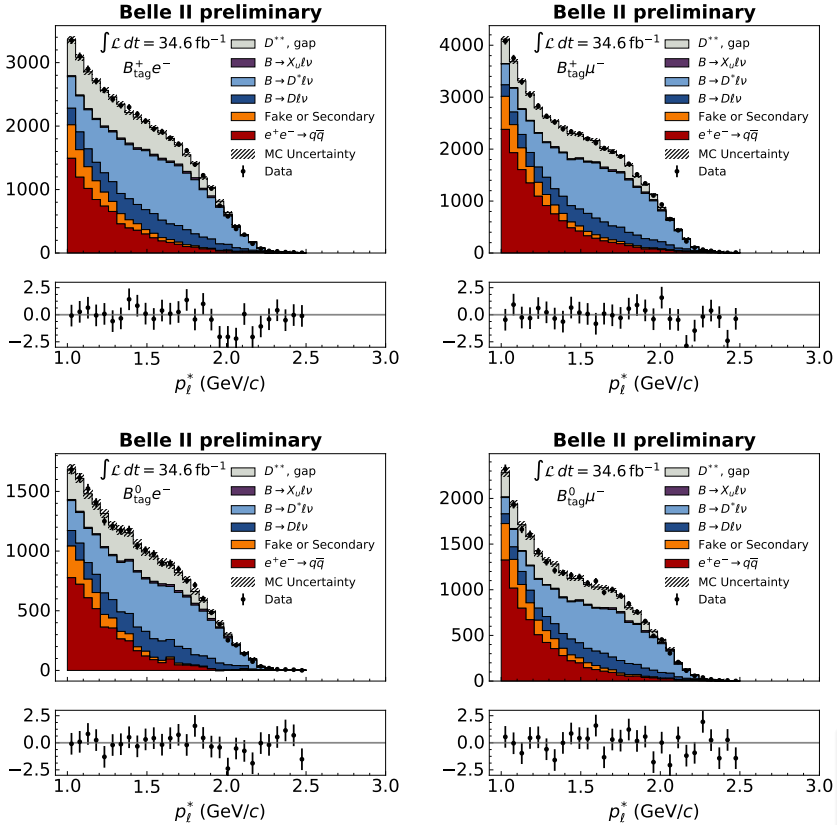
\includegraphics[width=0.8\textwidth]{figures/data_sim_corrections/tag_calibration.png}
        }
    }
    \subcaptionbox{\label{fig:fei_calib_bplusmuminus}}{
        \clipbox*{{0.5\width} {0.5\height} {1\width} {1\height}}{%
            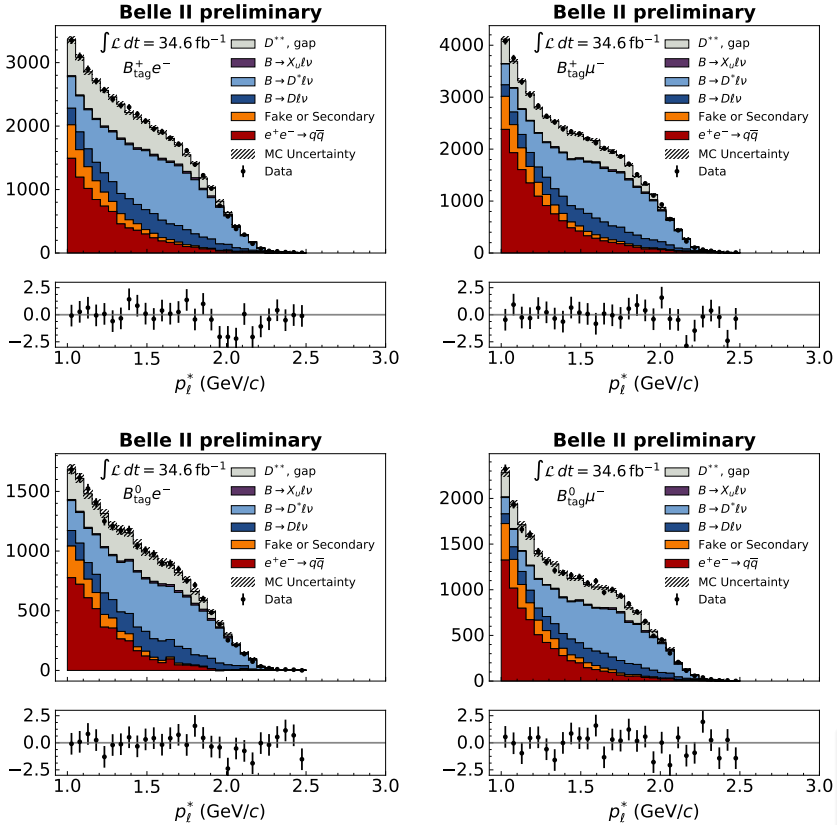
\includegraphics[width=0.8\textwidth]{figures/data_sim_corrections/tag_calibration.png}
        }
    }
    \subcaptionbox{\label{fig:fei_calib_bzeroeminus}}{
        \clipbox*{{0\width} {0\height} {0.5\width} {0.5\height}}{%
            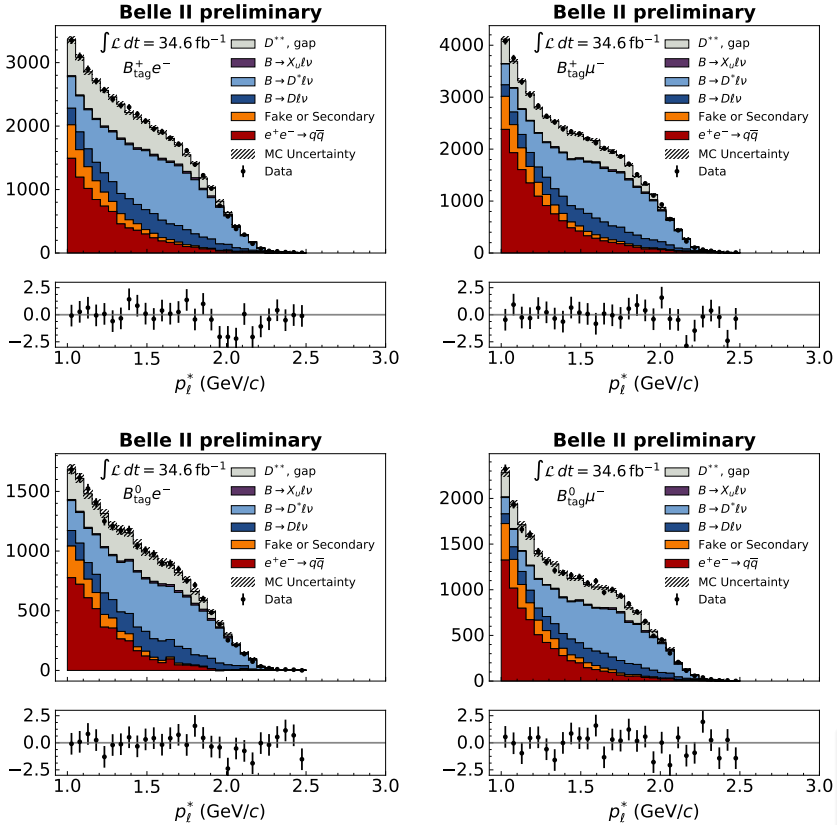
\includegraphics[width=0.8\textwidth]{figures/data_sim_corrections/tag_calibration.png}
        }
    }
    \subcaptionbox{\label{fig:fei_calib_bzeromuminus}}{
        \clipbox*{{0.5\width} {0\height} {1\width} {0.5\height}}{%
            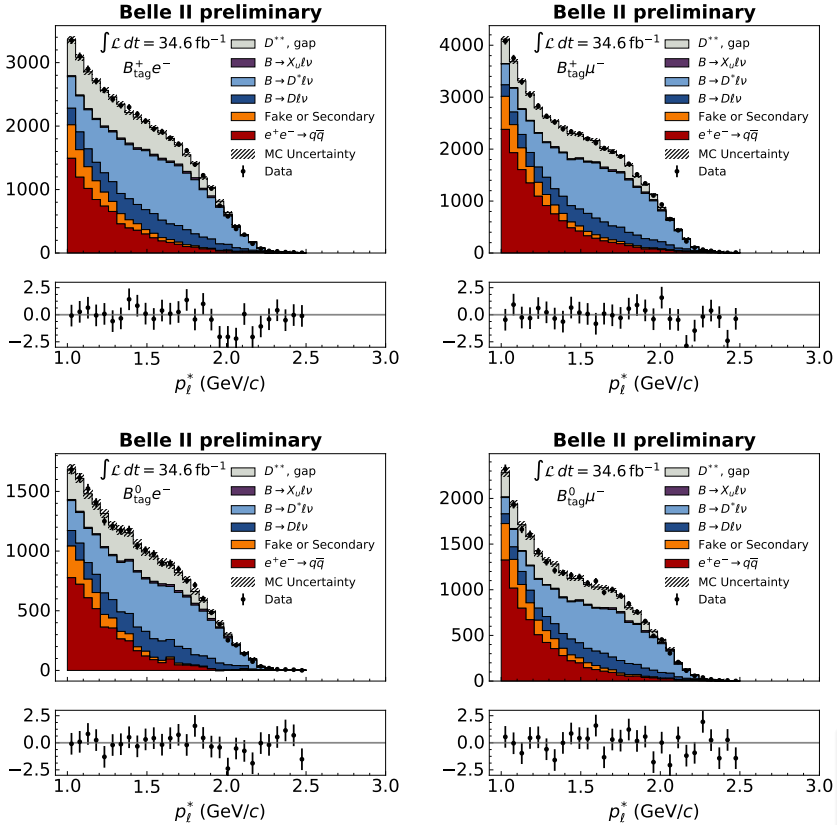
\includegraphics[width=0.8\textwidth]{figures/data_sim_corrections/tag_calibration.png}
        }
    }
    \caption{\label{fig:fei_calib} Illustration of the fits to \B\to$X_{u,c}\ell\nu$ decays in the \FEI calibration study.
    Results for the combinations of charged and neutral tag-$B$ modes with $e^-$ and $\mu^-$
    are shown in \Cref{fig:fei_calib_bpluseminus,fig:fei_calib_bplusmuminus,fig:fei_calib_bzeroeminus,fig:fei_calib_bzeromuminus}.
    Different fit components are shown in the legend and the subpanels contain the pulls of the fit.
    Figures taken from \cite{Belle-II:2020fst}.
    }
\end{figure}

Branching fractions of $B\rightarrow X_{u,c}\ell\nu$ are evaluated from the fitted distributions.
These values are then directly compared with the experimentally known values of branching fractions of these decays.
A correction factor, $\mathcal{C}_{\mathrm{FEI}}$ is derived, such that the two values are compatible.
The leading evaluated systematic uncertainties are found to be the imperfect experimental knowledge of the $B\rightarrow X_u\ell\nu$ branching fractions and their form factors, the fit model composition, tracking and particle identification uncertainties.
For the Belle II simulation campaign used in this analysis and averaged for both lepton modes, the result is as follows:
\begin{equation}\label{eq:fei_calibration}
    \mathcal{C}_{\mathrm{FEI}}(B^+) = 0.6599 \pm 0.225; \quad \mathcal{C}_{\mathrm{FEI}}(B^0) = 0.6695 \pm 0.0237,
\end{equation}
where two different calibration factors are presented for \feiBp and \feiBz modes, respectively.
Therefore, for an adequate comparison with Belle II data, any Belle II simulation involving the use of \FEI will be henceforth scaled appropriately.

\subsection{Calibration of \texorpdfstring{\piz}{pi0} and \texorpdfstring{$\eta$}{eta} suppression tools}\label{sec:piz_eta_calibration}
It was seen in \Cref{sec:selection_vetos}, that one of the strongest tools for background suppression in this analysis is the $\piz$ and $\eta$ suppression tool.
Consequentially, any data-simulation discrepancies will have a high impact on the final result.
The calibration of the \piz and $\eta$ is performed in an independent study and is not part of original work presented in this thesis.
For clarity, the calibration study is discussed in this Section.
\etaVeto calibration is henceforth implied, although only \piVeto is mentioned, as their calibration is equivalent.
Althrough the calibration study only studies \piVeto, it is assumed that the corrections are also valid for \etaVeto selections.

The main concern for this analysis is the primary (signal) photon efficiency: the number of photons that do not originate in light-meson decays and get rejected given a certain \piVeto selection.

The calibration study uses $B^+\to \bar{D}^0[\to K^+\pi^-]\pi^+$ decays and $B^0\to D^-[\to K^+\pi^-\pi^-]\pi^+$, where the square brackets denote a subdecay of the $D$ meson.
The $pi^+$, originating in the primary $B$ decay, is combined with all other photon candidates in the event, in a strategy described in \Cref{sec:selection_vetos}.
This produces many `\piz'-like combinations ($\mathit{pseudo-\piz}$) which yield a \piVeto score with minimal background from real \piz decays.

The reconstruction requires all charged tracks to have good-quality tracks that originate near the interaction point.
The identification information from Belle II subdetectors is used to distinguish pions and kaons.
Because $\pi^+$ from the primary $B$ decay is combined with other photons, a massless hypothesis is used for calculations of invariant mass and the helicity angles for the MVA.
After constructing the pseudo-\piz, selections on \piVeto are performed, corresponding to selections chosen in the analysis.
Therefore a distribution with no \piVeto selection, and a subset distribution with $\piVeto<0.4$ are created.
In both cases the charged and neutral $B$ channels are combined.

An unbinned \Mbc fit is performed on distributions with and without the \piVeto selections.
The \Mbc is modelled by a Crystal Ball function for signal decays and ARGUS function for continuum background.
All parameters of Crystal Ball and continuum are unconstrained.
An additional \PDF to model the peaking non-signal \BB components are used.
This \PDF is initialised in simulation, as a sum of a Gaussian and an Argus.
The shape parameters, and normalisation of this \BB background \PDF are not estimated, but kept at the initialised values.
The fits on data in the case of no \piVeto selection, and a $\piVeto<0.95$ selection are given in \Cref{fig:pivetofit}.
\begin{figure}[htbp!]
    \centering
    \subcaptionbox{\label{fig:pivetofit_nocut}}{
    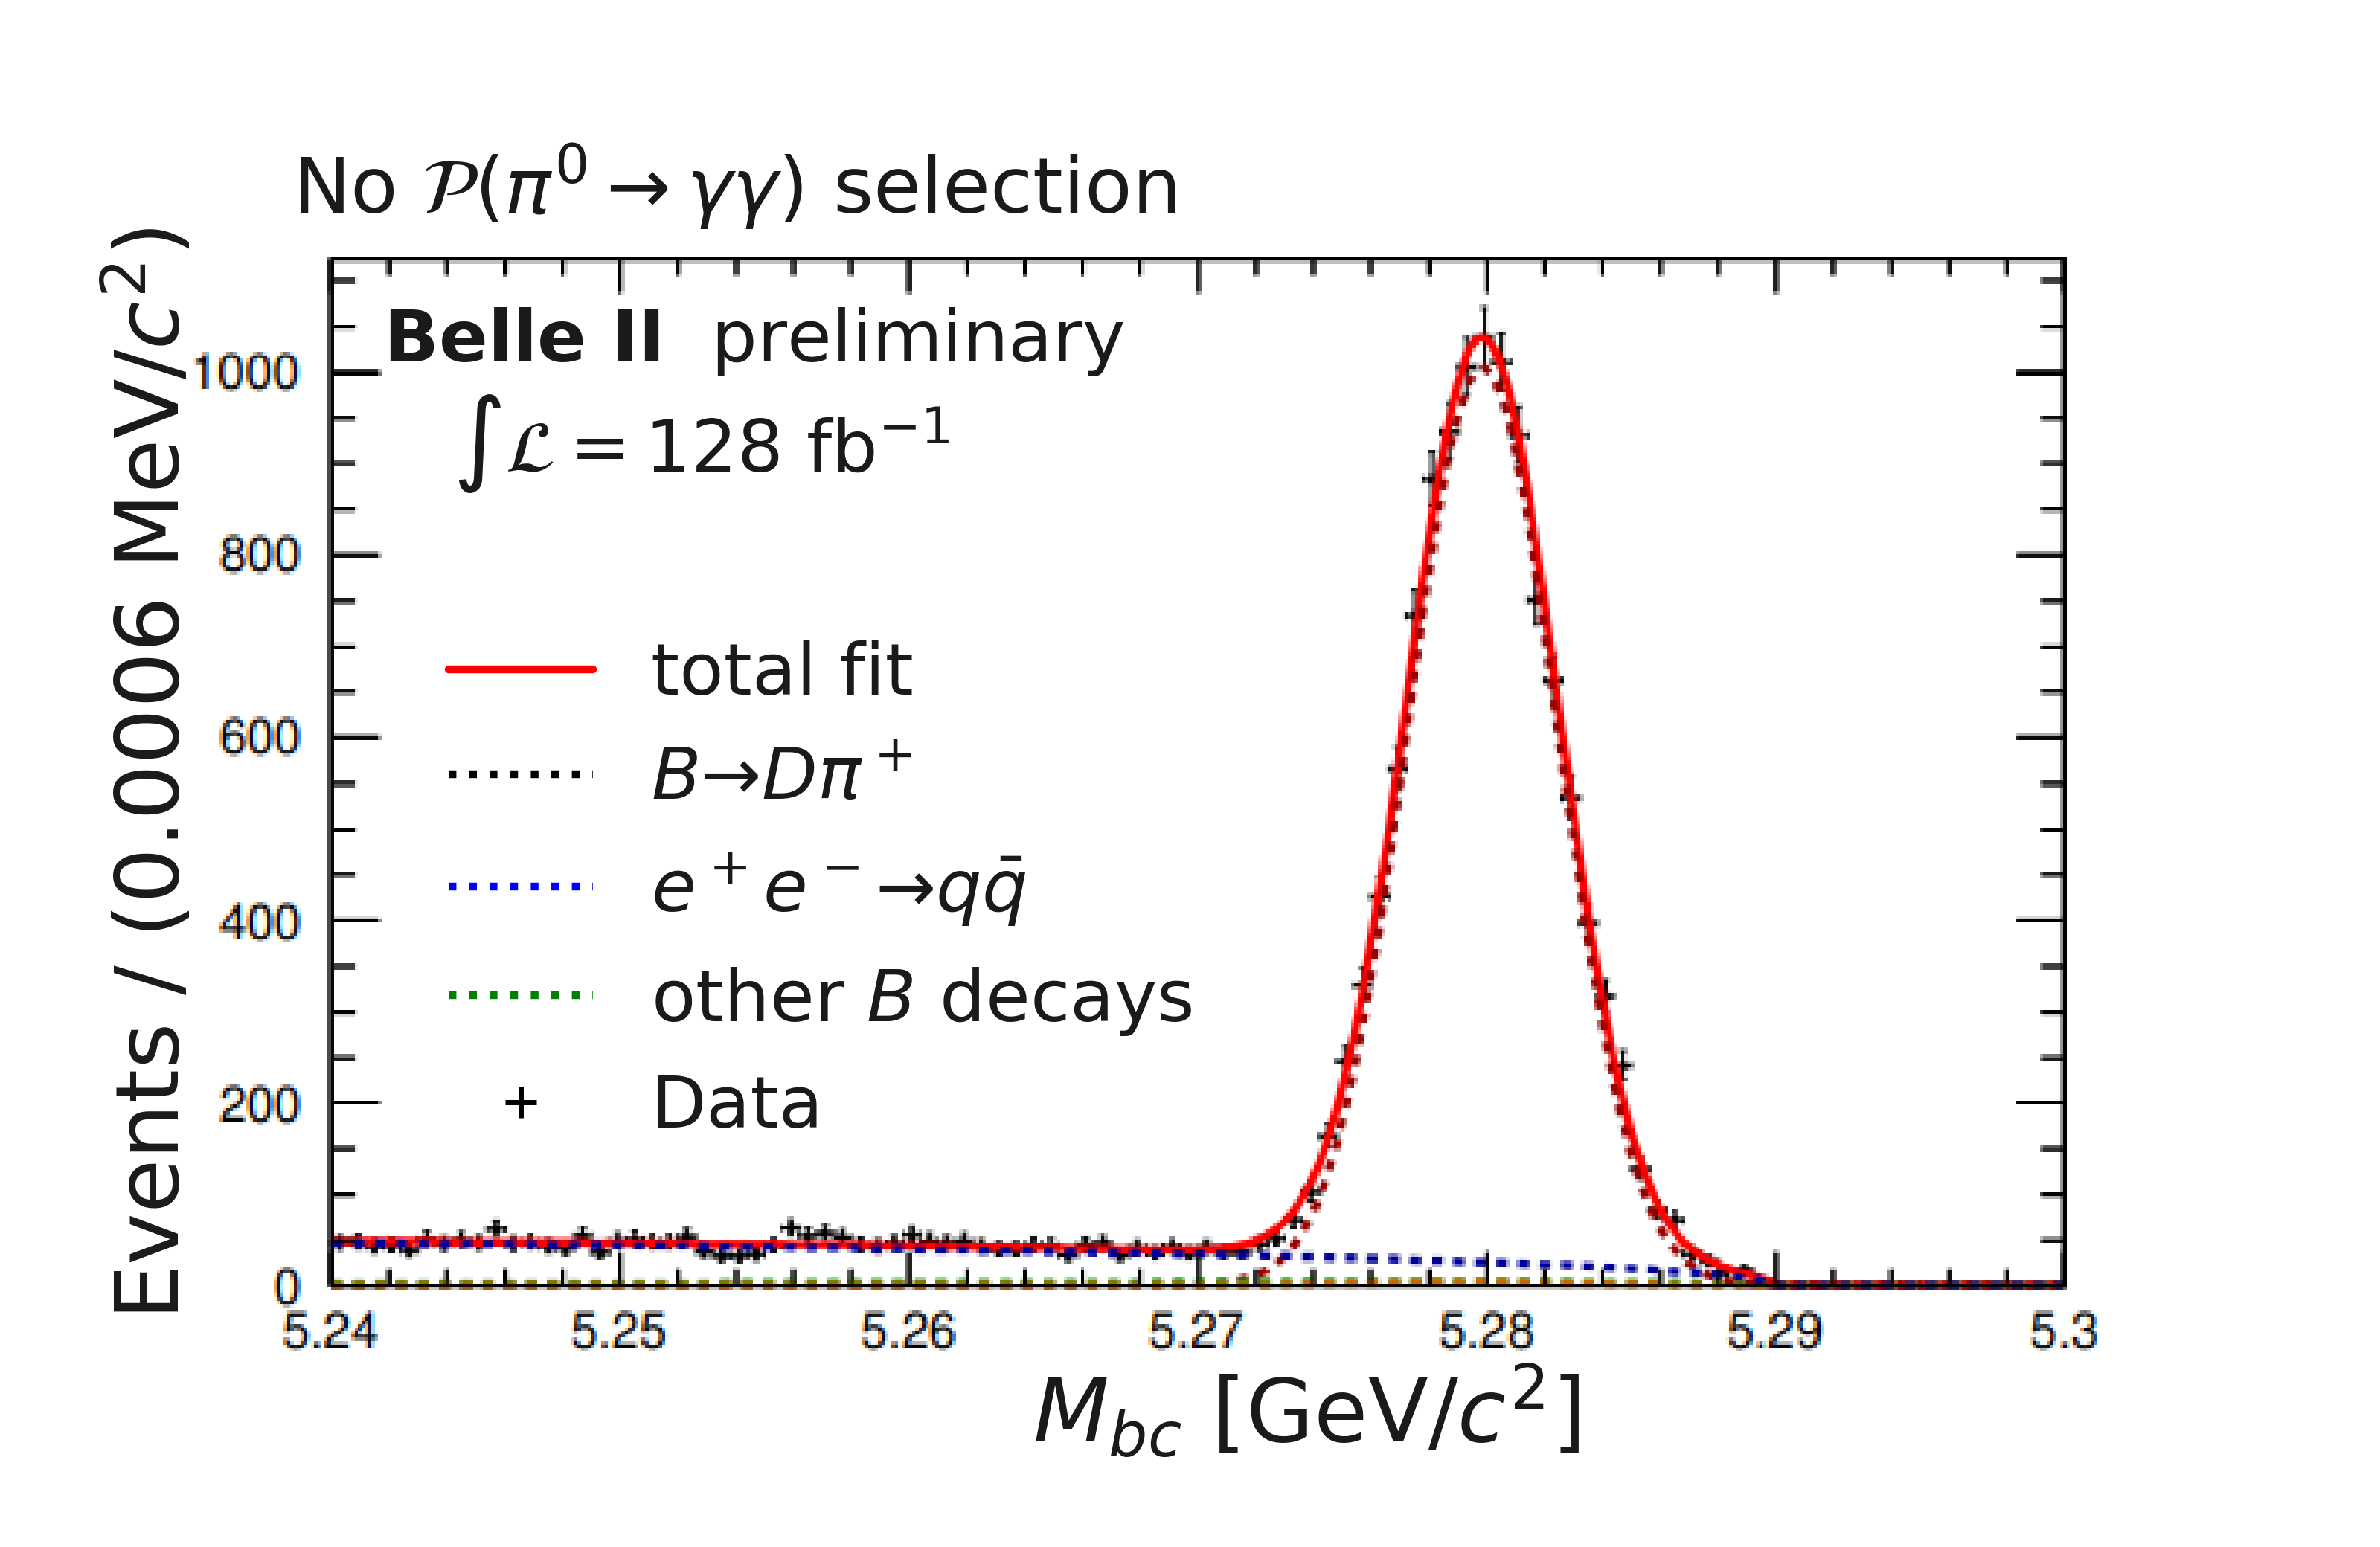
\includegraphics[width=0.4\textwidth]{figures/data_sim_corrections/data_fit_pi0_no_cut.png}
    }
    \subcaptionbox{\label{fig:pivetofit_cut}}{
        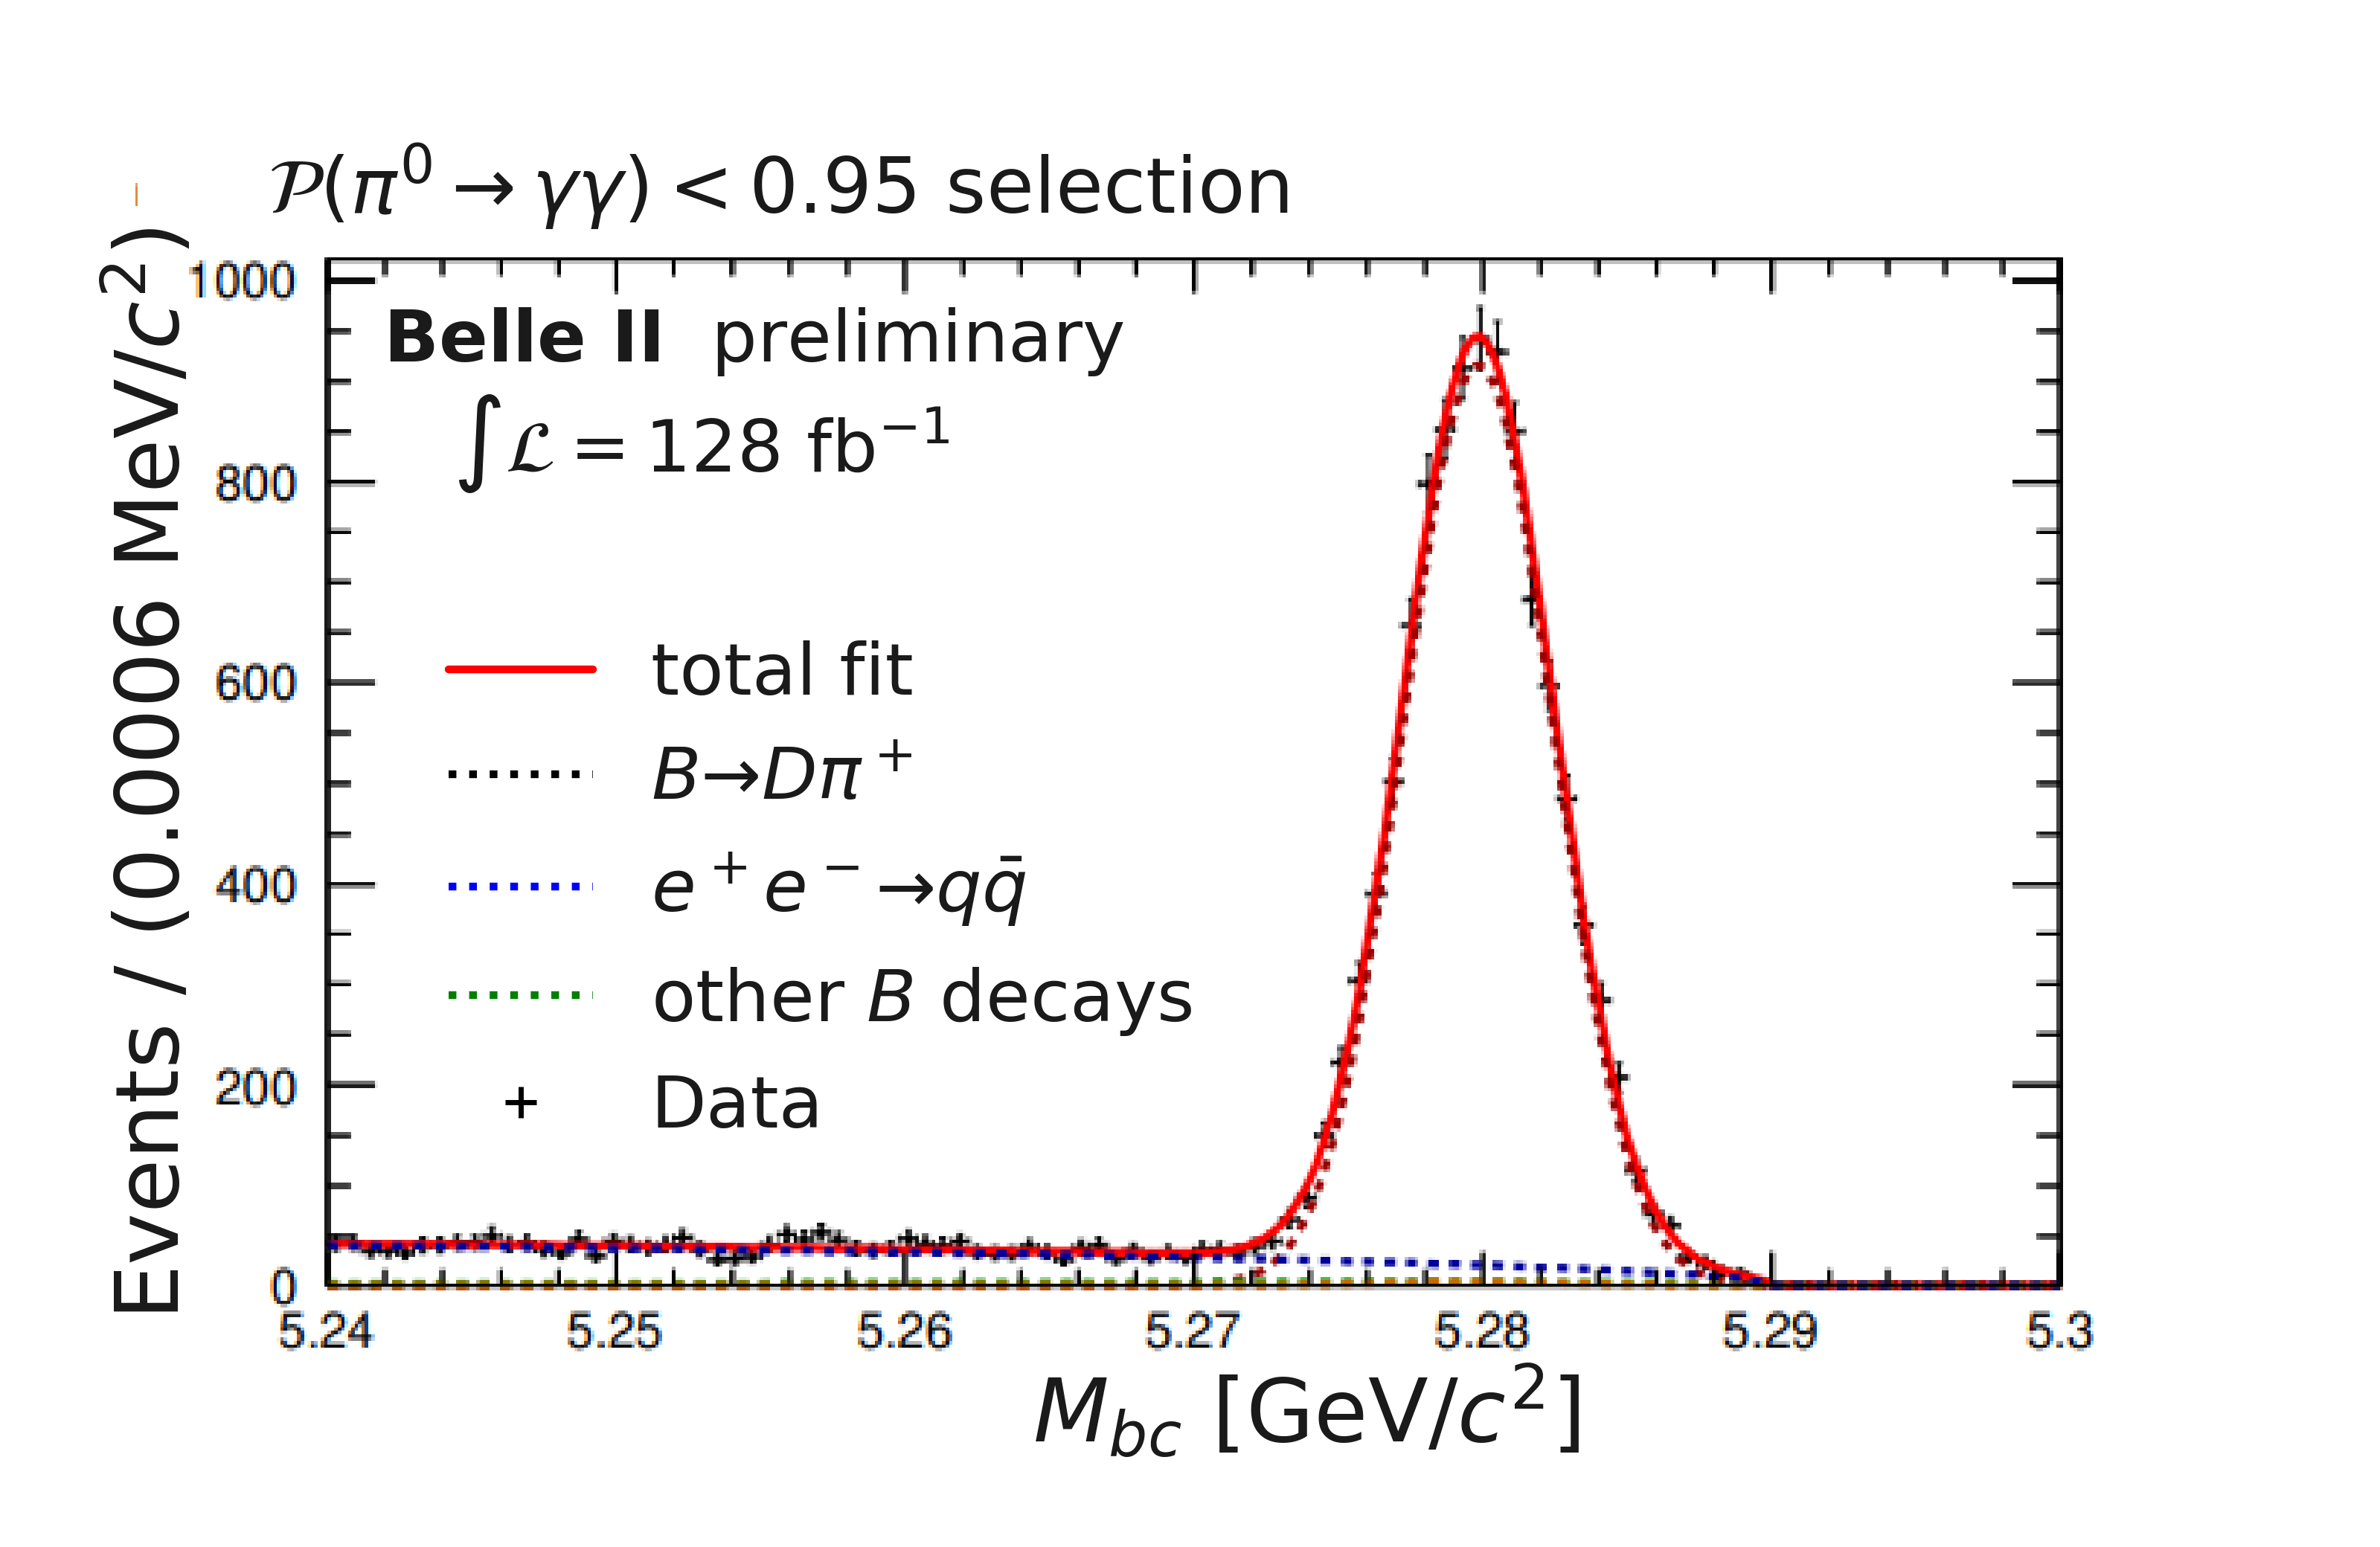
\includegraphics[width=0.4\textwidth]{figures/data_sim_corrections/data_fit_pi0_with_cut.png}
        }
    \caption{\label{fig:pivetofit} The fit estimating the number of $B\to D \pi^+$ events in Belle II data.
    Different \PDF{s} used in the fit are shown in the legend and explained in text.
    The fit is performed on a sample without (\Cref{fig:pivetofit_nocut}) and with (\Cref{fig:pivetofit_cut}) \piVeto selection applied.
    The extracted values from simulation and data are then combined to calculate \piVeto correction factors (see \Cref{eq:piveto_correction}).
    These figures are produced by a Belle II internal study of the \piz veto, and not part of the original work in this thesis.
    Only the labels and legends have been adapted.    
    }
\end{figure}

The fit extracts the counts of $B\to D\pi^+$ events, $N_{B\to D\pi^+}$ as the normalisation parameter of the Crystal Ball.
An efficiency, $\varepsilon\equiv N_{B\to D\pi^+}/N^{\piVeto<0.4}_{B\to D\pi^+}$ is defined, which corresponds to the primary-photon efficiency.
If the fit is performed in simulation (\MC) and data, an efficiency ratio can be used as a correction factor:
\begin{equation}\label{eq:piveto_correction}
    R_{\piVeto} = \frac{N_{B\to D\pi^+}/N^{\piVeto<0.4}_{B\to D\pi^+}|_{\mathrm{data}}}{N_{B\to D\pi^+}/N^{\piVeto<0.4}_{B\to D\pi^+}|_{\mathrm{MC}}}.
\end{equation}
The corrections are calculated in $200~\mev$ intervals of the lab-frame energy of the primary $\pi^+$.
The results for the selection chosen in this analysis are given in \Cref{fig:piveto_corrections}.
The internal Belle II study providing these corrections was only performed in the range of 1.8 to 3.0 ~\gev in the laboratory frame energy of the primary $\pi^+$.
Therefore, a linear extrapolation based is performed to estimate the value for values outside the range.
It is observed that the linear extrapolation is consisttent, within errors, with the corrections in the $1.8-3.0~\gev$.
Therefore, a correction factor of $1.1\pm0.5$ is chosen for events outside the range covered by the calubration study.
This value is consistent with all other correction factors.
\begin{figure}[htbp!]
    \centering
    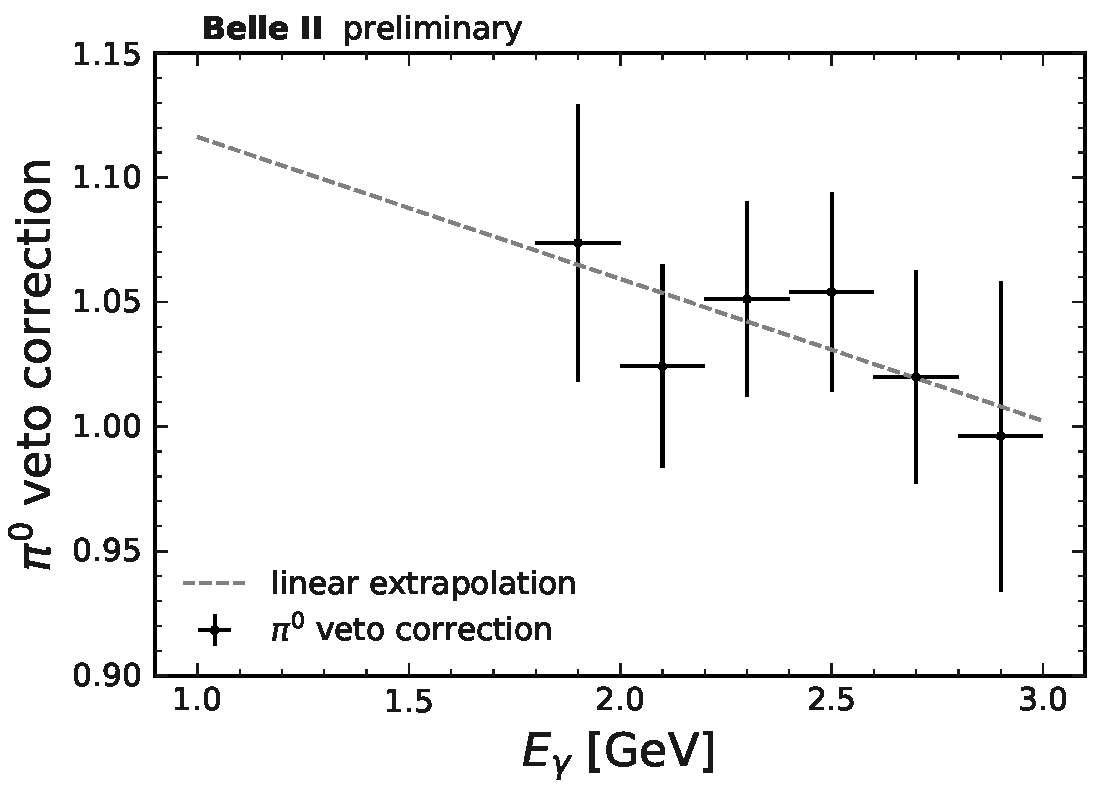
\includegraphics[width=0.45\textwidth]{figures/data_sim_corrections/pi0veto_corrections.pdf}
    \caption{\label{fig:piveto_corrections} The corrections $R_{\piVeto}$ for the $\piVeto<0.4$ selection used in this analysis.
    The results cover $1.8-3.0~\gev$ energies in the \textit{laboratory frame}, $\Egamma$.
    Because the laboratory frame energies cannot be trivially transformed to the $B$ meson rest-frame energies, a linear extrapolation to lower energies is performed.
    For missing $\Egamma$ phase space, in this analysis a $1.1\pm0.5$ value is adopted.
    }
\end{figure}

\subsection{Belle II calorimeter photon detection efficiency}\label{sec:photon_efficiency}

One of the main necessities of a measurement involving photons in the final state, is, of course, a precise and accurate simulation of the electromagnetic calorimeter -- the main tool of neutral particle detection.
In Belle~II, the \ECL provide this function.
Although it is known that its precision and resolution are excellent suited for flavour physics studies, exact data/simulation differences have to be known.
As part of the original work presented in this thesis, a Belle~II calorimeter photon detection efficiency study has been performed.
The initial setup of the analysis has been prepared by Dr. Natalia Kovalchuk and Dr. Torben Ferber, but I have updated the procedure, reworked the covered
and performed the full systematic uncertainty evaluation during my doctoral studies.
It is a critical study for the \BtoXsgamma analysis, however, the results of this study are also routinely used in other analyses that utilise photons in their final states.
The study is summarised in a Belle II public note \cite{Henrikas:2604}.
Here, the main measurement concepts and the results relevant to the measurement of \BtoXsgamma are presented.

To measure the photon detection efficiency, one must first have the knowledge that a photon has been created in an event, and then search for it within the calorimeter.
In this efficiency study $\epem\ra\mumu$ scattering events are employed.
In particular, collision events where a high energy photon is radiated in the initial state are sought.
The concept of the efficiency measurement is sketched in \Cref{fig:photon_efficiency_measurement}.
\begin{figure}[htbp!]
    \centering
    \subcaptionbox{\label{fig:eemumugamma_feynman}}{
    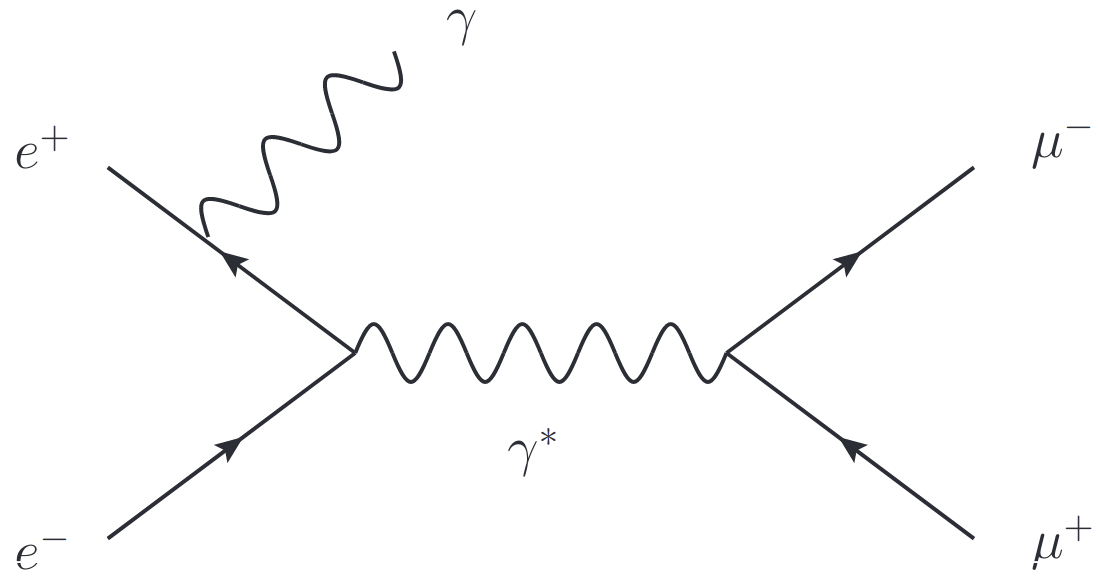
\includegraphics[width=0.4\textwidth]{figures/data_sim_corrections/eemumugamma.png}
    }
    \subcaptionbox{\label{fig:measurement_principle_gammaeff}}{
        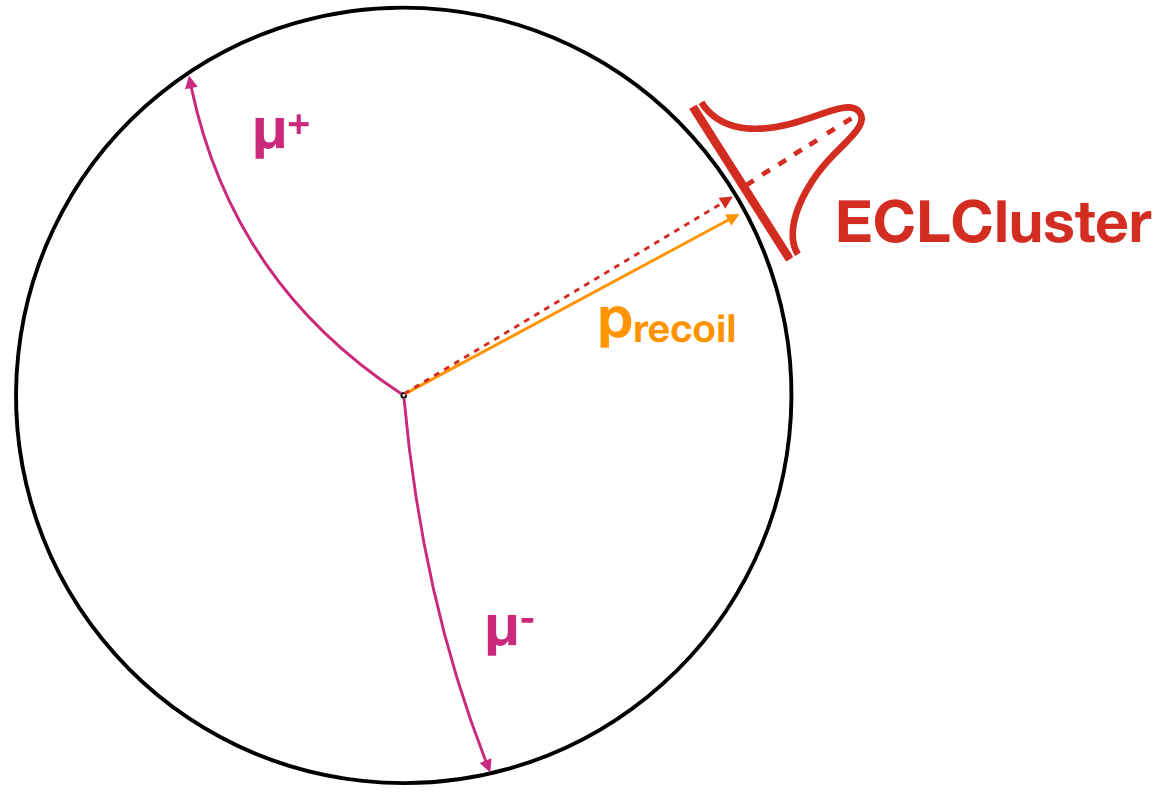
\includegraphics[width=0.4\textwidth]{figures/data_sim_corrections/measurement_principle.png}
        }
    \caption{\label{fig:photon_efficiency_measurement} The main concepts of the measurement of the Belle II photon detection efficiency.
    The \Cref{fig:eemumugamma_feynman} shows the Feynman diagram of the $\epem\ra\mumu$ events, where an photon is radiated in the initial collision state.
    Due to the radiated photon, the resulting dimuon system will have missing momentum with respect to the usual collision energy $\sqrt{s}\approx10.58~\gev$.
    The direction of the missing momentum can be extrapolated to search for photon clusters in the calorimeter, as sketched in \Cref{fig:measurement_principle_gammaeff}.
    \Cref{fig:measurement_principle_gammaeff}
    }
\end{figure}

The main goal is to reconstruct two muon tracks in each event and evaluate their total momentum and energy.
Because the high-energy photon (further called initial-state radiation or \ISR) is created before the collision, the energy of the dimuon system will have a certain degree of missing-momentum, whose direction will coincide with that of the emitted photon.
This missing momentum direction is called \textit{recoil}, and is charactarised by the magnitude (equivalent to the photon energy), polar angle and the azimuthal angle.
Therefore, by selecting events where such recoil are present, one is able to look for photon clusters corresponding to the angle and the energy within the calorimeter.
This gives a photon detection efficiency estimate through a simple event counting relation:
\begin{equation}\label{eq:photon_efficiency}
    \varepsilon_{\gamma}(|\vec{p}_{\mathrm{recoil}}|, \theta_{\mathrm{recoil}}, \phi_{\mathrm{recoil}}) = \frac{N(\mathrm{photon~found}~\cup~\mathrm{recoil~found})}{N(\mathrm{recoil~found})},
\end{equation}
which can be evaluated as a function of missing momentum, with a magnitude $|\vec{p}_{\mathrm{recoil}}|$ and corresponding angles $\theta$ and $\phi$.

Many background processes may degrade the efficiency by producing events with sufficient recoil momentum.
A notable example are the $\epem\ra\tautau$ events which may produce two muons and four neutrinos through subsequent $\tau$ decays.
The presence of neutrinos create a missing momentum which can fake that originating from an \ISR photon.
Furthermore, tracking inefficiencies can lead to an incorrect measurement of the direction or magnitude of the recoil vector.
Finally, instances where not one, but two or more \ISR events occur can complicate the photon finding procedure, resulting in an overall drop of efficiency.
Therefore, \Cref{eq:photon_efficiency} is more correctly referred to as \textit{photon finding efficiency}, rather than photon detection efficiency.

These photon finding inefficiency effects are suppressed to a certain degree through a double ratio measurement:
\begin{equation}\label{eq:photon_data_mc}
    R_{\gamma} = \frac{\varepsilon_{\gamma}^{\mathrm{DATA}}}{\varepsilon_{\gamma}^{\mathrm{MC}}},
\end{equation}
where $\varepsilon_{\gamma}$ are respective values of photon finding efficiency calculated in data or simulation, based on \Cref{eq:photon_efficiency}.
The double ratio, $R_{\gamma}$, is considered the photon detection efficiency data-to-simulation ratio in this analysis.

First, tracks consistent with $\epem\ra\mumu$ processes are selected by requiring each event to have exactly two charged tracks that:
\begin{itemize}
    \item have straight, high-energy tracks, which is ensured by a high-momentum requirement $p>1~\gevc$;
    \item are consistent to have originated from the interection point;
    \item act as a minimum ionising particle in the \ECL: leave energy deposits smaller than 300~\mev and less than 80\% of the total momenta.
\end{itemize}
The two muon tracks passing these requirements are used to evaluate the missing energy and momentum of the event, requiring the recoil magnitude $p_{\mathrm{recoil}}>0.2~\gevc$.
Backgrounds from various $\epem\ra\mathrm{hadrons}$ or $\epem\ra\tautau$ are strongly suppressed by the mass associated to the missing momentum requirement,
$m^2_{\mathrm{Recoil}}<2~\gev/c^4$. 
Additional checks, such as sufficient isolation of the muon tracks and recoil are required to ensure adequate separation between their energy deposits in the \ECL.
If all the aforementioned requirements are passed, an event is considered to have a \textit{recoil found}.
\todo[inline]{talk a bit why m2recoil is useful here}
The distributions for events with a recoil found are shown in \Cref{fig:selected_photon_data_mc}.

The photon candidates are selected by requiring them to have a center-of-mass energy of at least $75~\mev$ and a timing of the associated cluster at $\pm200~\ns$.
These requirements were optimised to reduce the impact of beam background photons and leftover photons from previous collisions.
No tighter selections on photons or their reconstruction quality is made, to ensure that no bias is introduced in the detection efficiency.

The recoil candidates are matched to photon clusters in the \ECL via two matching requirements:
\begin{itemize}
    \item Photons have to be within 0.3~\rad radial cone around the recoil direction;
    \item The cluster energy to recoil momentum ratio must satisfy $1.2>E_{\gamma}/\pRecoil>0.5$.
\end{itemize}
If both requirements are fulfilled the event is considered to have a \textit{photon found}.
The distribution of events where a recoil is sucessfully matched to a photon are given in \Cref{fig:matched_photon_data_mc}.
\begin{figure}[htbp!]
    \centering
    \subcaptionbox{\label{fig:selected_photon_data_mc}}{
    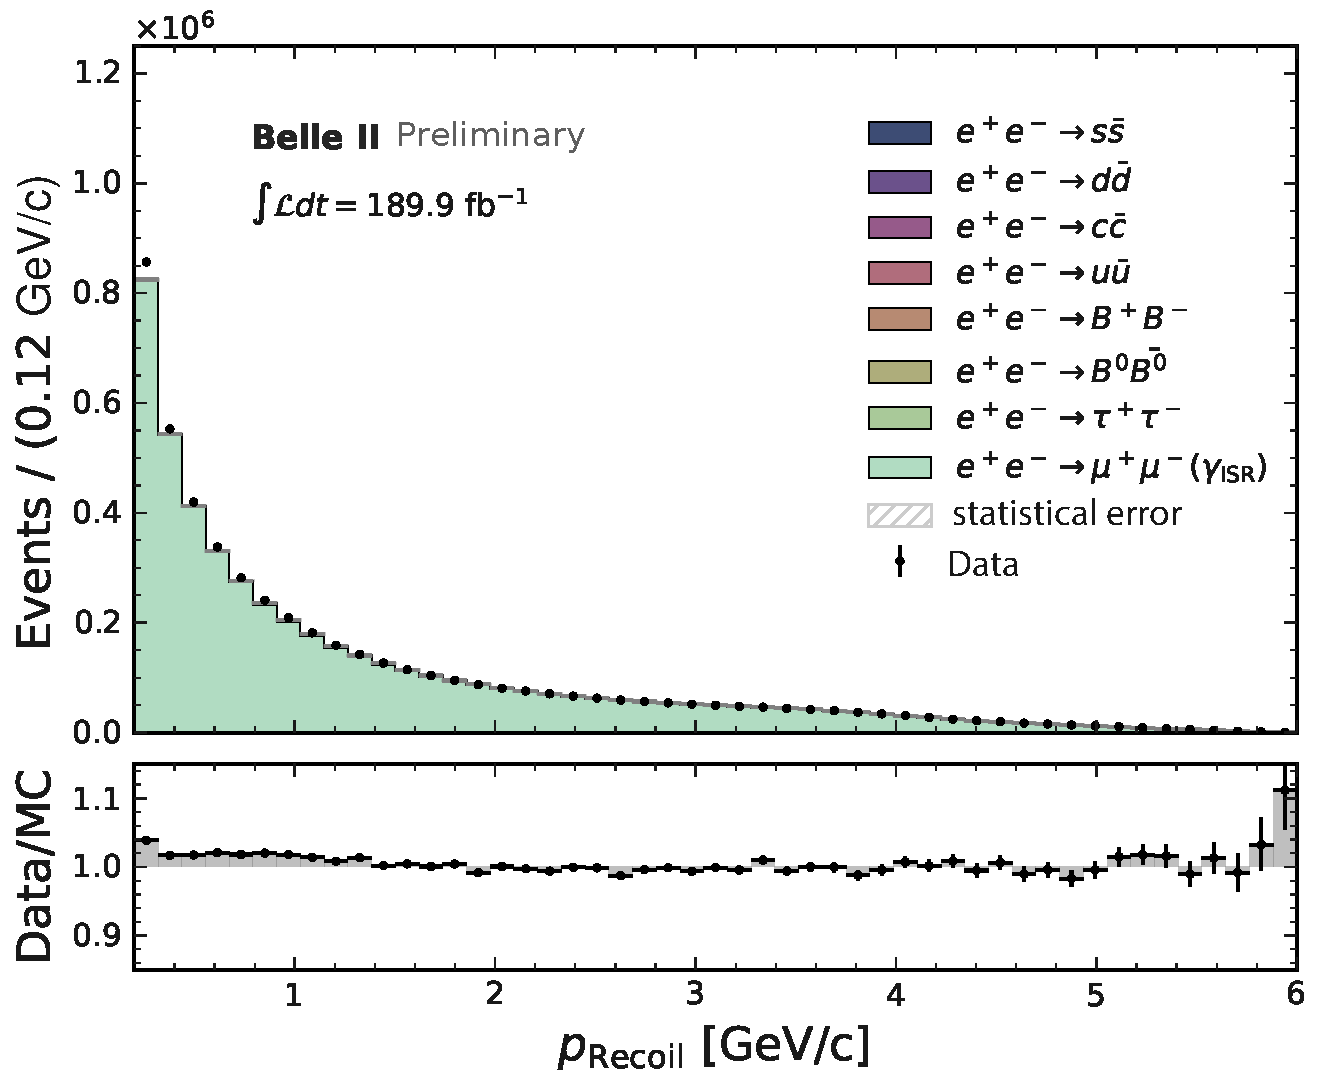
\includegraphics[width=0.4\textwidth]{figures/data_sim_corrections/pyth_data_normalisation_to_mc_comparison_pRecoil_selected.pdf}
    }
    \subcaptionbox{\label{fig:matched_photon_data_mc}}{
        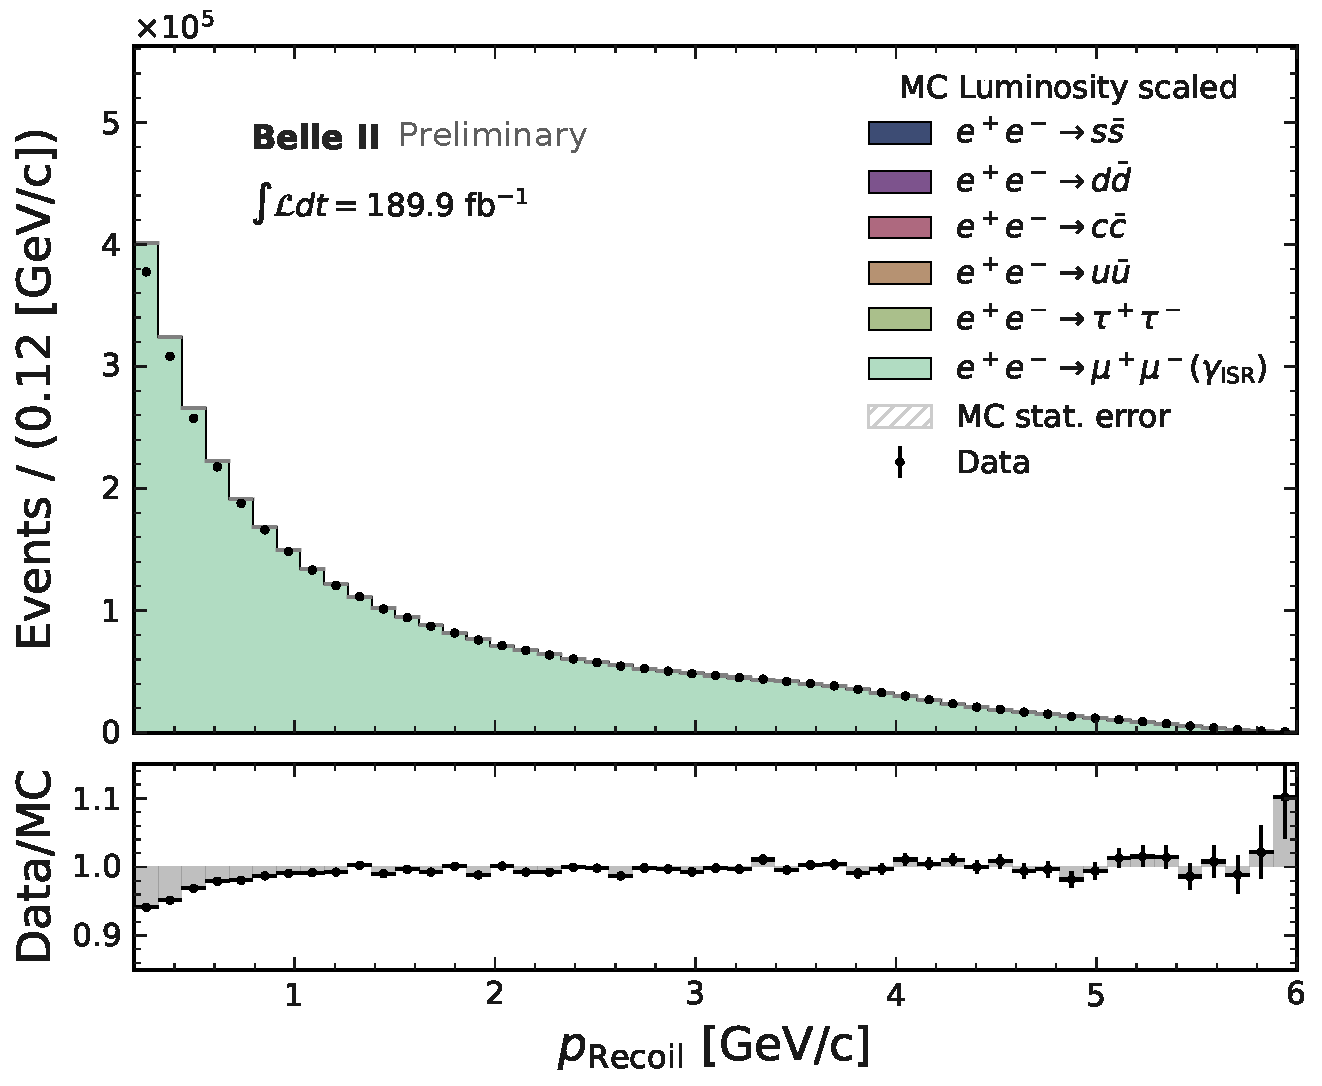
\includegraphics[width=0.4\textwidth]{figures/data_sim_corrections/pyth_data_normalisation_to_mc_comparison_pRecoil_matched.pdf}
    }
    \caption{\label{fig:normalisation_data_mc} Distribution of $\epem\ra\mumu$ events, with a photon radiated in the initial interaction state, as a function of the magnitude of the missing momentum of the dimuon system (which corresponds to the energy of the radiated photon).
    \Cref{fig:selected_photon_data_mc} shows events where a missing momentum has been found.
    \Cref{fig:matched_photon_data_mc} shows events where a missing momentum has been found and it was consistent with photon in the calorimeter, as discussed in the text.
    Various sources of background events are also included, and they can be seen to be at very low level.
    Overall, the signal and background events describe data accurately.
    The subpanels show the data-to-simulation ratio.
    These figures contain only statisical uncertainties.
    The figures show results for the datasets of size equivalent to the ones used in this analysis.
    \todo[inline]{I need to modify labels in one of these (free trial expired)}
    }
\end{figure}

The events represented in \Cref{fig:selected_photon_data_mc} correspond to the numerator of \Cref{eq:photon_efficiency}, whereas the \Cref{fig:matched_photon_data_mc} -- to the denominator.
Finding efficiencies are calculated and their ratio in data and simulation are simulation.
In simulation, only $\epem\ra\mumu$ events are used for the finding efficiency.
The measured backgrounds, particularly the most prominent $\epem\ra\tautau$ background, is subtracted from the data distributions.
The results are shown in \Cref{fig:data_mc_photon_eff}.
The data-to-simulation ratio is generally high and approximately equal to unity for photons above 1~\gev.
A drop-off for low-energy photons (low-\pRecoil) is attributed to the presence of soft \ISR photons in the event which affect the direction of the recoil.
This effect becomes larger with the lower photon energy.
\begin{figure}[htbp!]
    \centering
    \includegraphics[width=0.45\textwidth,page=2]{figures/data_sim_corrections/pyth_data_mc_agreement_pRecoil.pdf}
    \caption{\label{fig:data_mc_photon_eff} The photon finding efficiency as a function of missing momentuom of the dimuon system, \pRecoil.
    The subpanel shows the ratio of of data and simulation finding efficiencies, as per \Cref{eq:photon_data_mc}.
    All figures includes systematic uncertainties, which are correlated between data and simulation.
    The figures show results for the datasets of size equivalent to the ones used in this analysis.
    }
\end{figure}

The systematic uncertainties are also calculated.
Most of the selections are tightened and loosened to evaluate the dependance of the efficiency on selection requirements.
The maximum shifts in the central value are assigned as systematic uncertainties.
A full shift to the central value without remaining background subtraction from data is also added as a systematic uncertainty.
The largest systematic uncertainties arise from leftover background modelling, $m^2_{\mathrm{Recoil}}$ selection variations, and muon calorimeter energy deposit variation requirements,
but in total they are at $\order(1\%)$ level.

Equivalent distributions to \Cref{fig:normalisation_data_mc} as 3-D functions of \pRecoil, \pRecoilPhi and \pRecoilTheta are produced and 3-D efficiency maps are calculated.
Based on the detected photon direction and energy, appropriate corrections are applied.
In the \BtoXsgamma analysis, the event-level information is lost after performing the \Mbc fit and subtracting the remaining \BB background.
Therefore the average corrections are evaluated in \BtoXsgamma hybrid-signal model based on the \EB spectrum binning.
These value are provided in \Cref{tab:correction_table}.

\subsection{Modelling of remaining-\texorpdfstring{\BB}{BB} background processes}

While the results of previous sections correct for the procedures used in the removal of photon and tag-side backgrounds, they do not account for any discrepancies that may be introduced when generating the simulated datasets.
Although a full study of all possible background modes that may contribute to the leftover-\BB background is, likely, a subject for another full doctoral thesis, the adequacy of background simulation was studied for the purposes of the analysis presented here.
In general, Belle~II simulation is validated and known to produce accurate and precise simulation of most processes that are common to $B$ factories.
However, our knowledge of Nature and the Standard Model is constantly improving, therefore the branching fractions or other parameters used in the generation of the generic-\BB simulation may not be updated in time, as the simulation campaigns happen roughly yearly.
The goal of this study is to check that the generated branching fractions of the main backgrounds that contribute to \BtoXsgamma match those reported by the Particle Data Group \cite{Workman:2022ynf}.

First, only events contributing to good tag-\B mesons based on studies in \Cref{sec:good_tag_definition} are selected.
In each \EB interval, all (non-\BtoXsgamma) $B$ decay modes that produce high-energy photon candidates are selected.
The modes are ranked by their relative abundance (fraction) within that \EB interval.
Particularly in low-\EB region there are hundreds of different $B$ meson decay channels that can contribute to the background.
Pragmatically, only background $B$ decays that contribute at least 1\% to the background in at least one \EB interval are further considered.
These requirements encompass 53 \Bp modes and 39 \Bz decay modes. 
They are listed in \Cref{tab:leftover_bp} and \Cref{tab:leftover_bz}, respectively.
The table also contain their relative fraction in every given bin.
As there are hundreds of $B$ decay modes that contribute at $\order(<1\%)$ relative fraction, these requirements may not cover all background in low-\EB regions. 
However, it is assumed that the corrections for non-dominant background modes should on average be 1, as large branching fraction differences in Belle~II simulation are not expected.

Main source of background photons is various $B\to D$ transitions where photons originate from either subsequent $D$ decays or the accompanying particle, e.g. $B\to D\rho$.
Semileptonic $B$ decays are also a major source of background.
In general, $B\to D$ transitions are largely dominating up to $2.2-2.3~\gev$.
At higher \EB other types of decays become prominent, but rather sporadically, without clearly dominating modes.
In particular, various rare $B$ decays, such as $B\to K$, $B\to\pi$ and $B\to\eta$ transitions become more prominent.

The selected background $B$ decay modes have their branching fraction in the Belle~II simulation files compared with that reported by the Ref. \cite{Workman:2022ynf}.
Based on the findings, a following correction, for every mode in every \EB bin is derived:
\begin{equation}\label{eq:background_bf_correction}
    R^{B\ra X}_{\mathrm{BB}}(\EB) =  f(\EB) \times \frac{\mathcal{B}_{\mathrm{PDG}}}{\mathcal{B}_{\mathrm{Belle~II}}},
\end{equation}
where $f(\EB)$ is the relative fraction of a background mode $B\to X$ in a given \EB interval,
and $\mathcal{B}_{\mathrm{PDG}}$, $\mathcal{B}_{\mathrm{Belle~II}}$ denote the branching fractions found in the Particle Data Group summary (\cite{Workman:2022ynf}) and Belle~II simulation, respectively.
If available, the $\mathcal{B}_{\mathrm{PDG}}$ is varied according to the provided uncertainty, otherwise a 100\% variation is taken, and the central value shifts calculated with appropriate variations are assigned as uncertainties for $R^{B\ra X}_{\mathrm{BB}}(\EB)$.
The results are summed together and their uncertainties are propagated, taking the correlations, resulting from the fact that same decay mode may contribute in multiple \EB bins.
The correction factors from \Bp and \Bz background modes are averaged, assuming no correlation between different $B$ charges.
The final correction factors and their uncertainties are shown in \Cref{tab:correction_table}.
The values are (nearly) all consistent with unity, as expected considering the high-quality of the Belle~II simulation.

The correlation matrix of the correction factors arising from the fact that similar decay modes occur across many bins is shown in \Cref{fig:bbar_correlation_matrix}.
\begin{figure}[htbp!]
    \centering
    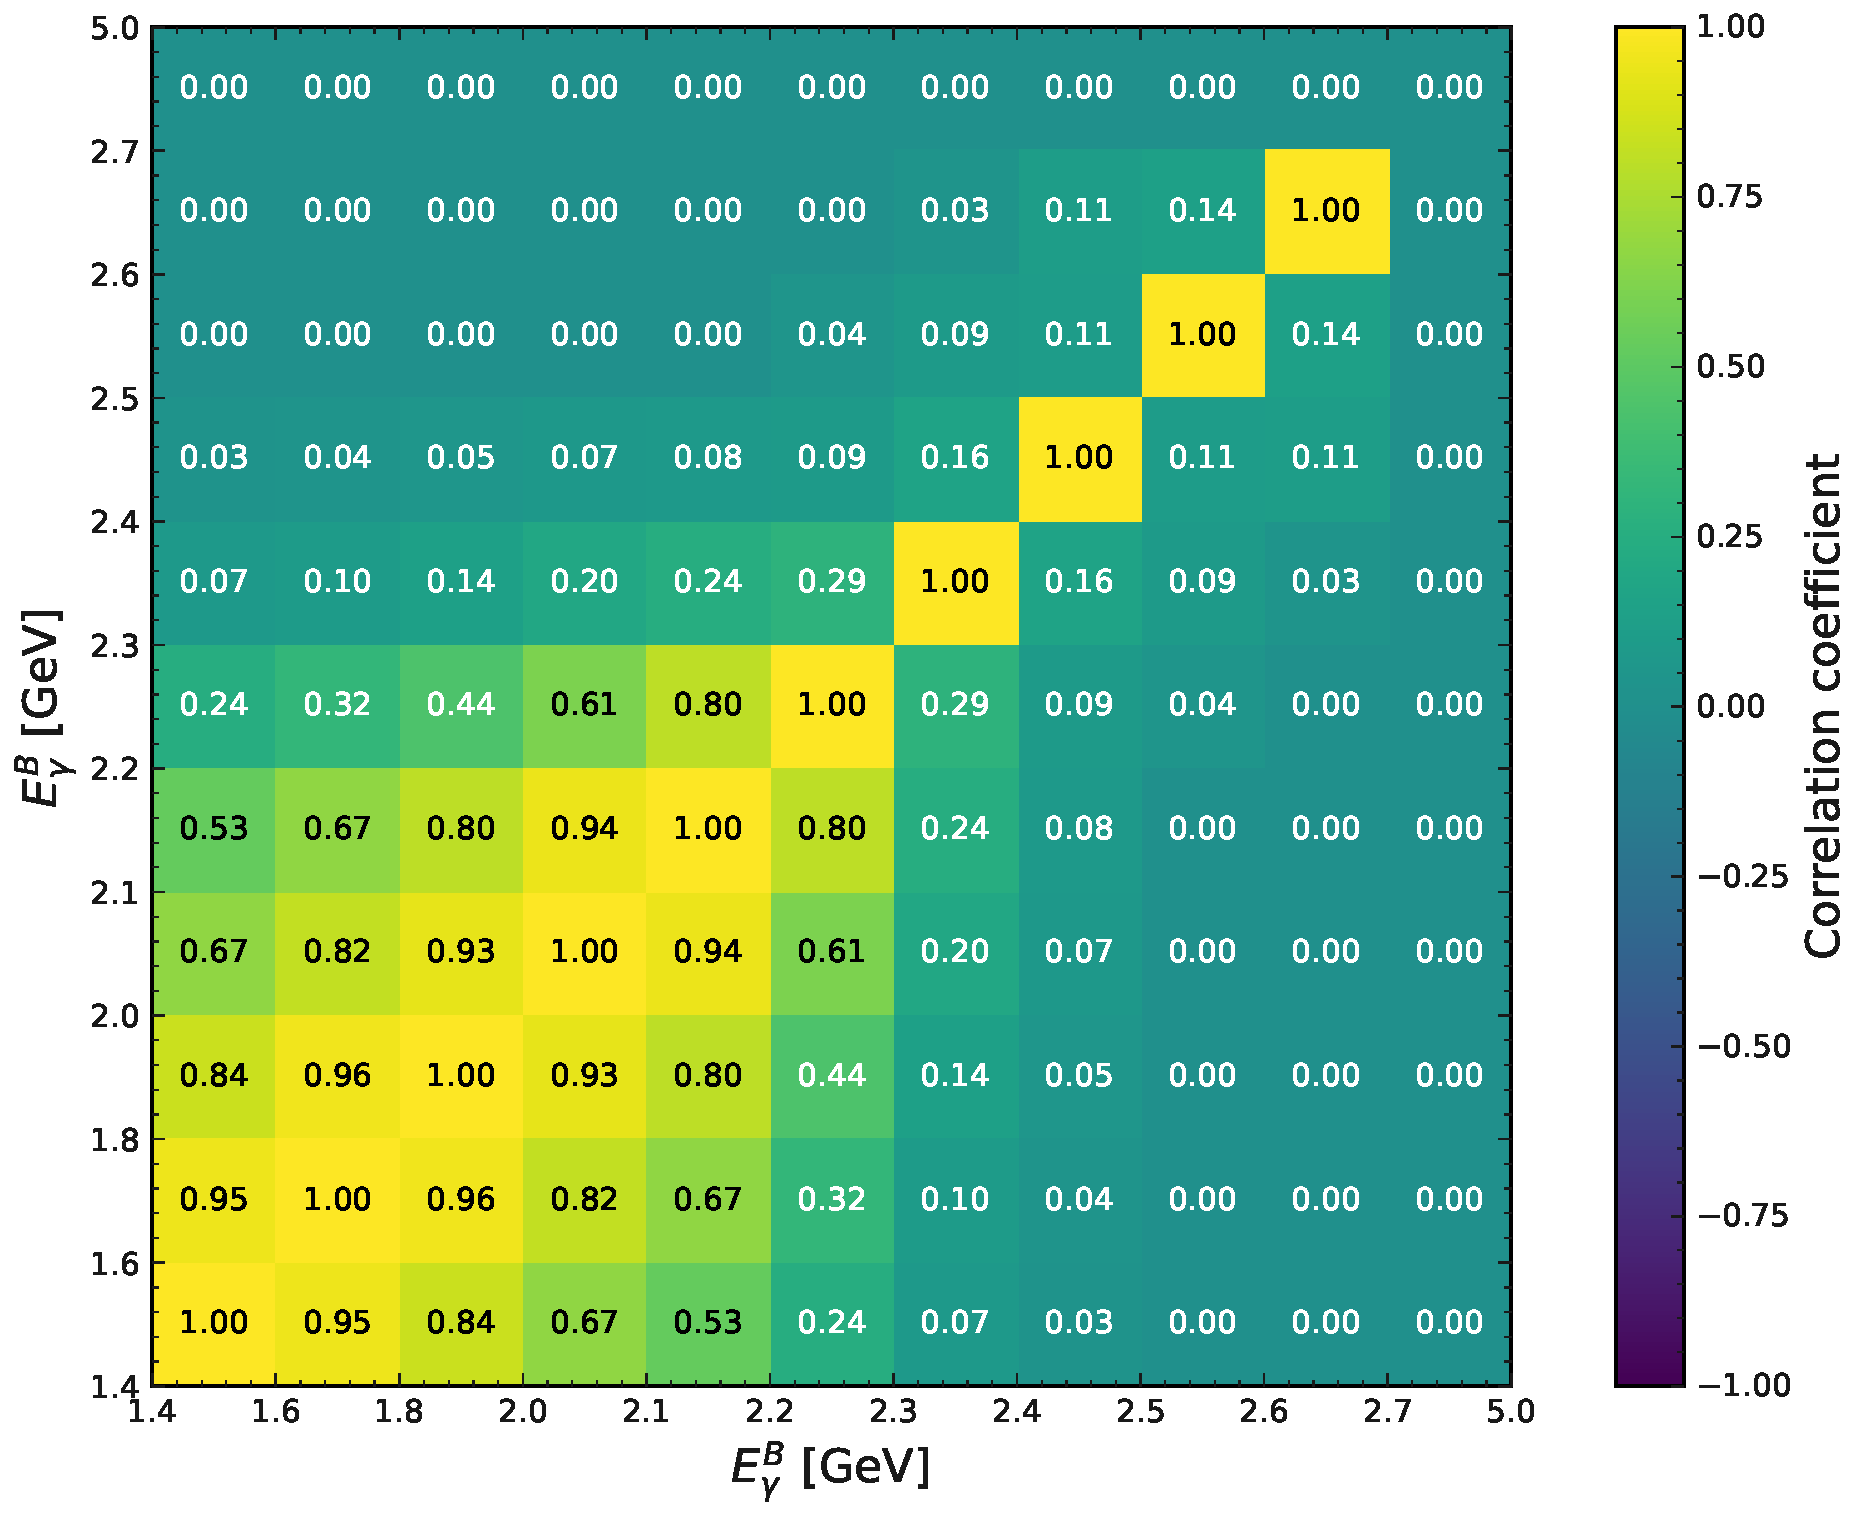
\includegraphics[width=0.5\textwidth]{figures/data_sim_corrections/bbar_correlation_matrix.pdf}
    \caption{\label{fig:bbar_correlation_matrix} The correlation matrix of \BB corrections.
    Particularly low-\EB bins are largely correlated due to the fact that similar background modes contribute in these regions.
    On the other hand, high-\EB background photons originate more sporadically and from fewer sources, thereby reducing the correlation.
    }
\end{figure}
It can be seen that mostly low-\EB bins are correlated, whereas high-\EB bins show smaller correlations.
This is attributed to the fact that abundant background processes fall off quickly with increasing \EB.
In the high-\EB region background photons are rarer and often originate as outliers from various CKM-suppressed decays, which decorrelates the bins.

\subsection{Out-of-time photon suppression}\label{sec:out_of_time_photon_suppression}

Although no special corrections are calculated, an additional selection is added to ensure that photons from beam background and previous collision events are not included in the analysis.
It is known that these effects are not well captured by the Belle~II run-period independent simulation that was used in this analysis.
Therefore, a timing selection requires the photon to be registered in a time-window $|\tau_{\gamma}|<200~\ns$ around the collision time.
Furthermore, to reject poorly reconstructed photons, a $|\tau_{\gamma}|/\Delta\tau_{\gamma}<2$ requirement is added, which suppresses photons with low-quality or failed cluster fits.
Using a technique analogous to $\epem\ra\mumu$ recoil study, it is observed that it degrades the photon finding efficiency by less than 2\%.
Therefore these selections are employed with no data-to-simulation correction.

\todo[inline]{review this, because this is nonsense.Maybe add beam background plots.}